\documentclass[11pt,a4paper]{article}
\usepackage[utf8]{inputenc}
\usepackage[T1]{fontenc}
\usepackage[brazilian]{babel}
\usepackage{geometry,graphicx,amsmath,amssymb,booktabs,tabularx,float,microtype}
\usepackage[hidelinks]{hyperref}
\geometry{margin=2cm}
\setlength{\parindent}{1.2em}
\setlength{\parskip}{4pt}
\setcounter{tocdepth}{2}

\title{\textbf{Tratando Incerteza em Monitoramento Inteligente}\\
\large Portfólio de Inteligência Artificial}
\author{
\textbf{Aluno:} Lucas Andrade Zanetti\\
\textbf{Matrícula:} 241039645\\
\textbf{Disciplina:} Inteligência Artificial\\
\textbf{Código:} FGA0221\\
\textbf{Professor:} Fabiano Araujo Soares
}
\date{4 de novembro de 2026}

\begin{document}
\maketitle
\thispagestyle{empty}
\begin{abstract}
Este relatório apresenta um portfólio integrado sobre tratamento de incerteza aplicado ao monitoramento de uma máquina industrial sujeita a ruído, variações operacionais e falhas. Foram desenvolvidos três projetos independentes em Python: uma Rede Bayesiana para diagnóstico probabilístico, um Modelo Markoviano Oculto (HMM) para identificação de estados operacionais ao longo do tempo e um Filtro de Kalman para estimação de variáveis físicas. As implementações centrais foram desenvolvidas manualmente, com validações, testes automatizados, dados sintéticos reproduzíveis e visualizações em alta resolução. Os resultados mostram que cada técnica responde a uma dimensão distinta do problema: relações causais e evidências, dinâmica temporal de estados ocultos e estimação contínua sob ruído.
\end{abstract}
\tableofcontents
\newpage

\section{Introdução e proposta}
Sistemas industriais modernos combinam sensores heterogêneos e decisões que precisam ser tomadas mesmo quando as medições são incompletas ou imprecisas. Temperatura, vibração, pressão e consumo energético não revelam diretamente o estado interno de uma máquina: são observações sujeitas a ruído e podem ser compatíveis com mais de uma causa. O objetivo deste portfólio é demonstrar, em um mesmo cenário, três formas complementares de representar e tratar essa incerteza.

O tema central é \textbf{monitoramento inteligente e diagnóstico de falhas em sistemas industriais}. A máquina considerada possui componentes sujeitos a desgaste, condições de sobrecarga e degradação da lubrificação. Os sintomas observados pelos sensores podem indicar falha mecânica ou elétrica, mas não determinam uma conclusão por si só. O portfólio foi organizado para responder a três perguntas:
\begin{enumerate}
\item Dadas evidências atuais, qual é a probabilidade de cada falha? (Rede Bayesiana.)
\item Qual foi a sequência mais provável de estados operacionais que produziu as observações? (HMM.)
\item Qual é a posição e a velocidade mais prováveis de um componente quando o sensor é ruidoso? (Kalman.)
\end{enumerate}

\subsection{Objetivos}
O objetivo geral é implementar e avaliar algoritmos probabilísticos capazes de apoiar manutenção preditiva. Os objetivos específicos são: (i) representar dependências causais por um grafo acíclico e realizar inferência exata; (ii) inferir estados ocultos em uma sequência temporal e estimar parâmetros por Baum--Welch; (iii) combinar modelo dinâmico e medições para obter uma estimativa filtrada; e (iv) avaliar limitações, sensibilidade e estabilidade numérica.

\section{Arquitetura e metodologia comum}
Os três projetos estão separados em diretórios, mas seguem uma metodologia comum. Os algoritmos principais estão em módulos próprios, os experimentos em arquivos separados e cada projeto possui uma entrada \texttt{main.py}. Os dados são sintéticos, pois permitem controlar as condições verdadeiras e medir o desempenho contra um gabarito conhecido. Todas as execuções relevantes usam sementes fixas: 19 no HMM e 23 no Kalman.

As figuras são produzidas com Matplotlib a 300 DPI. As métricas são salvas em arquivos JSON em \texttt{results/metrics.json}, o que evita transcrever resultados manualmente. Os testes automatizados verificam propriedades matemáticas centrais, incluindo normalização do Forward, validade de probabilidades, respeito a transições impossíveis, simetria da covariância e rejeição de dimensões incompatíveis.

\subsection{Critérios de avaliação}
No diagnóstico Bayesiano, foram comparadas probabilidades posteriores em quatro cenários e calculada uma variação de sensibilidade. No HMM, foram usadas acurácia, F1 macro, matriz de confusão e evolução da log-verossimilhança. No Kalman, foram usados RMSE e MAE da posição, além de uma comparação entre níveis de ruído e de uma hipótese incorreta para a covariância de medição.

\section{Projeto 1 — Rede Bayesiana}
\subsection{Modelagem do problema}
A rede possui oito variáveis binárias: desgaste (\textit{wear}), lubrificação insuficiente, sobrecarga, temperatura alta, vibração alta, pressão inadequada, falha mecânica e falha elétrica. Desgaste influencia a lubrificação; sobrecarga e lubrificação influenciam temperatura e pressão; desgaste e sobrecarga influenciam vibração. Os sintomas, por sua vez, contribuem para as hipóteses de falha.

\begin{figure}[H]
\centering
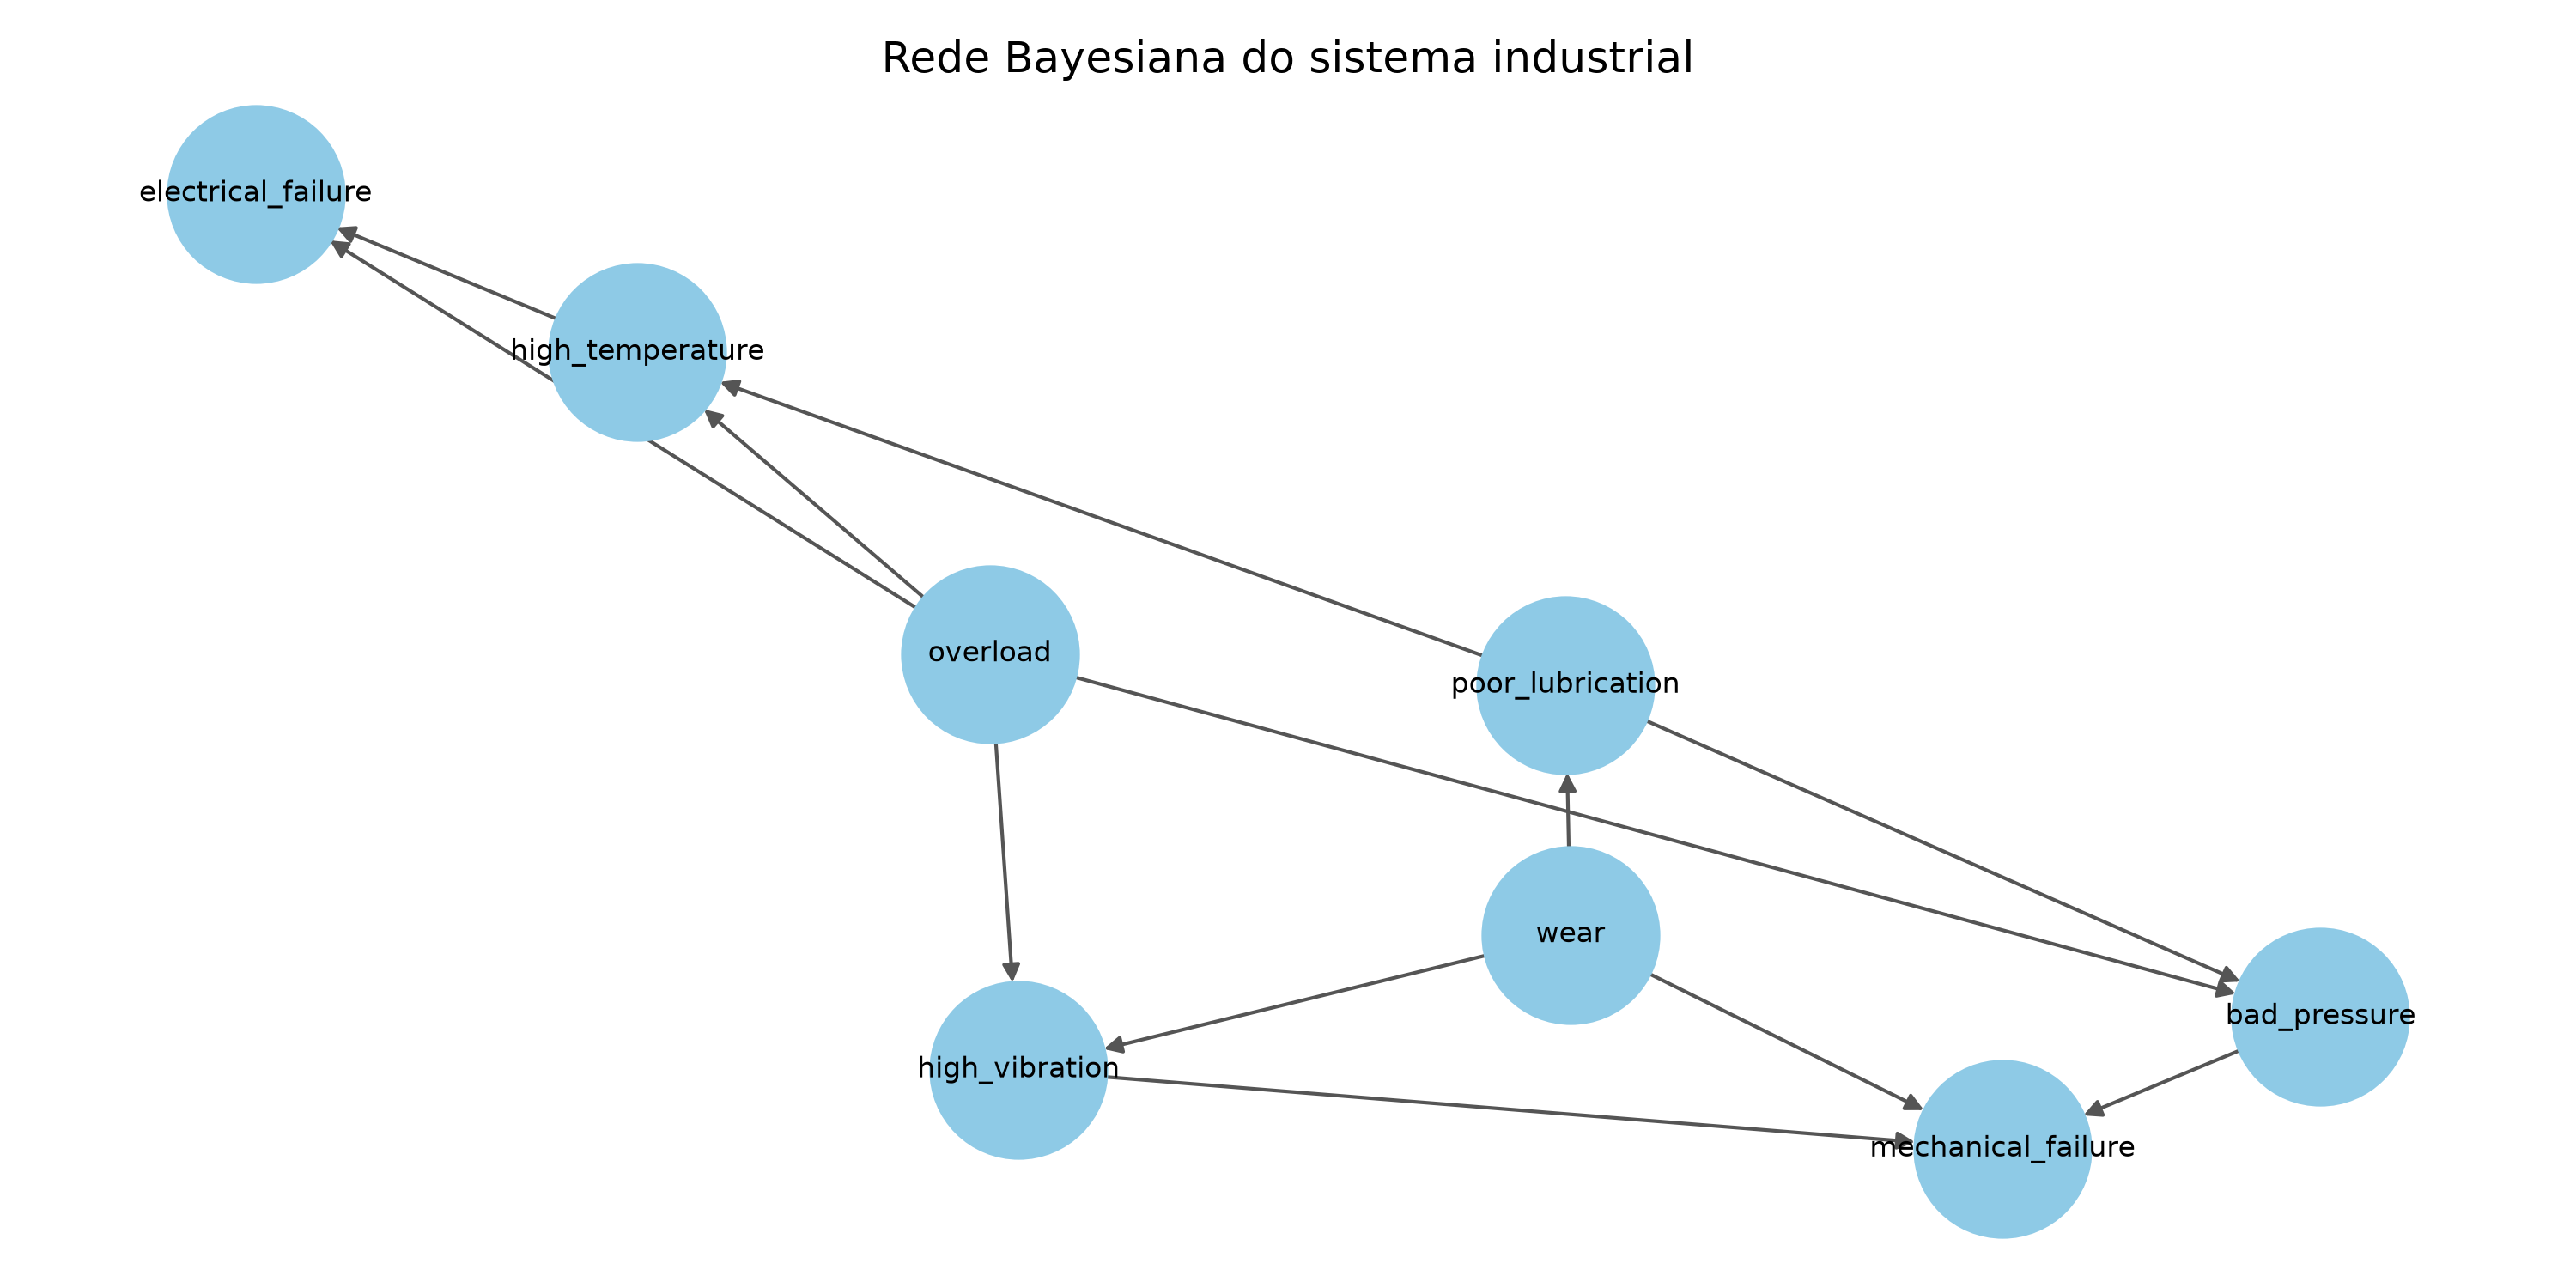
\includegraphics[width=.78\linewidth]{projeto_1_redes_bayesianas/results/bayesian_network.png}
\caption{Grafo acíclico direcionado da Rede Bayesiana.}
\end{figure}

Para uma atribuição completa $\mathbf{x}$, a distribuição conjunta é fatorada como
\[
P(\mathbf{x})=\prod_i P(x_i\mid \mathrm{pais}(X_i)).
\]
As probabilidades condicionais foram definidas manualmente para refletir o conhecimento do cenário: por exemplo, a probabilidade de vibração alta aumenta com desgaste e sobrecarga. O código verifica a existência de todos os nós, ausência de ciclos, completude das CPTs e validade das probabilidades.

\subsection{Inferência}
Para uma consulta $Q$ e evidência $\mathbf{e}$, foi implementada enumeração exata:
\[
P(Q\mid\mathbf{e}) =
\frac{\sum_{\mathbf{y}}P(Q,\mathbf{e},\mathbf{y})}
{\sum_{q,\mathbf{y}}P(q,\mathbf{e},\mathbf{y})}.
\]
Essa escolha é didática e adequada à rede pequena. Ela expõe diretamente a fatoração e o cálculo da distribuição posterior, sem ocultar o mecanismo em uma biblioteca pronta. Sua limitação é o crescimento exponencial com o número de variáveis.

\subsection{Resultados}
\begin{table}[H]\centering\small
\caption{Probabilidades posteriores produzidas pela execução.}
\begin{tabular}{lrrrr}
\toprule
Cenário & Falha mecânica & Falha elétrica & Desgaste & Sobrecarga\\
\midrule
Operação normal & 0,147 & 0,068 & 0,180 & 0,150\\
Temperatura e vibração altas & 0,628 & 0,445 & 0,552 & 0,715\\
Indícios elétricos & 0,036 & 0,308 & 0,159 & 0,346\\
Múltiplas evidências & 0,824 & 0,472 & 0,625 & 0,789\\
\bottomrule
\end{tabular}
\end{table}

\begin{figure}[H]
\centering
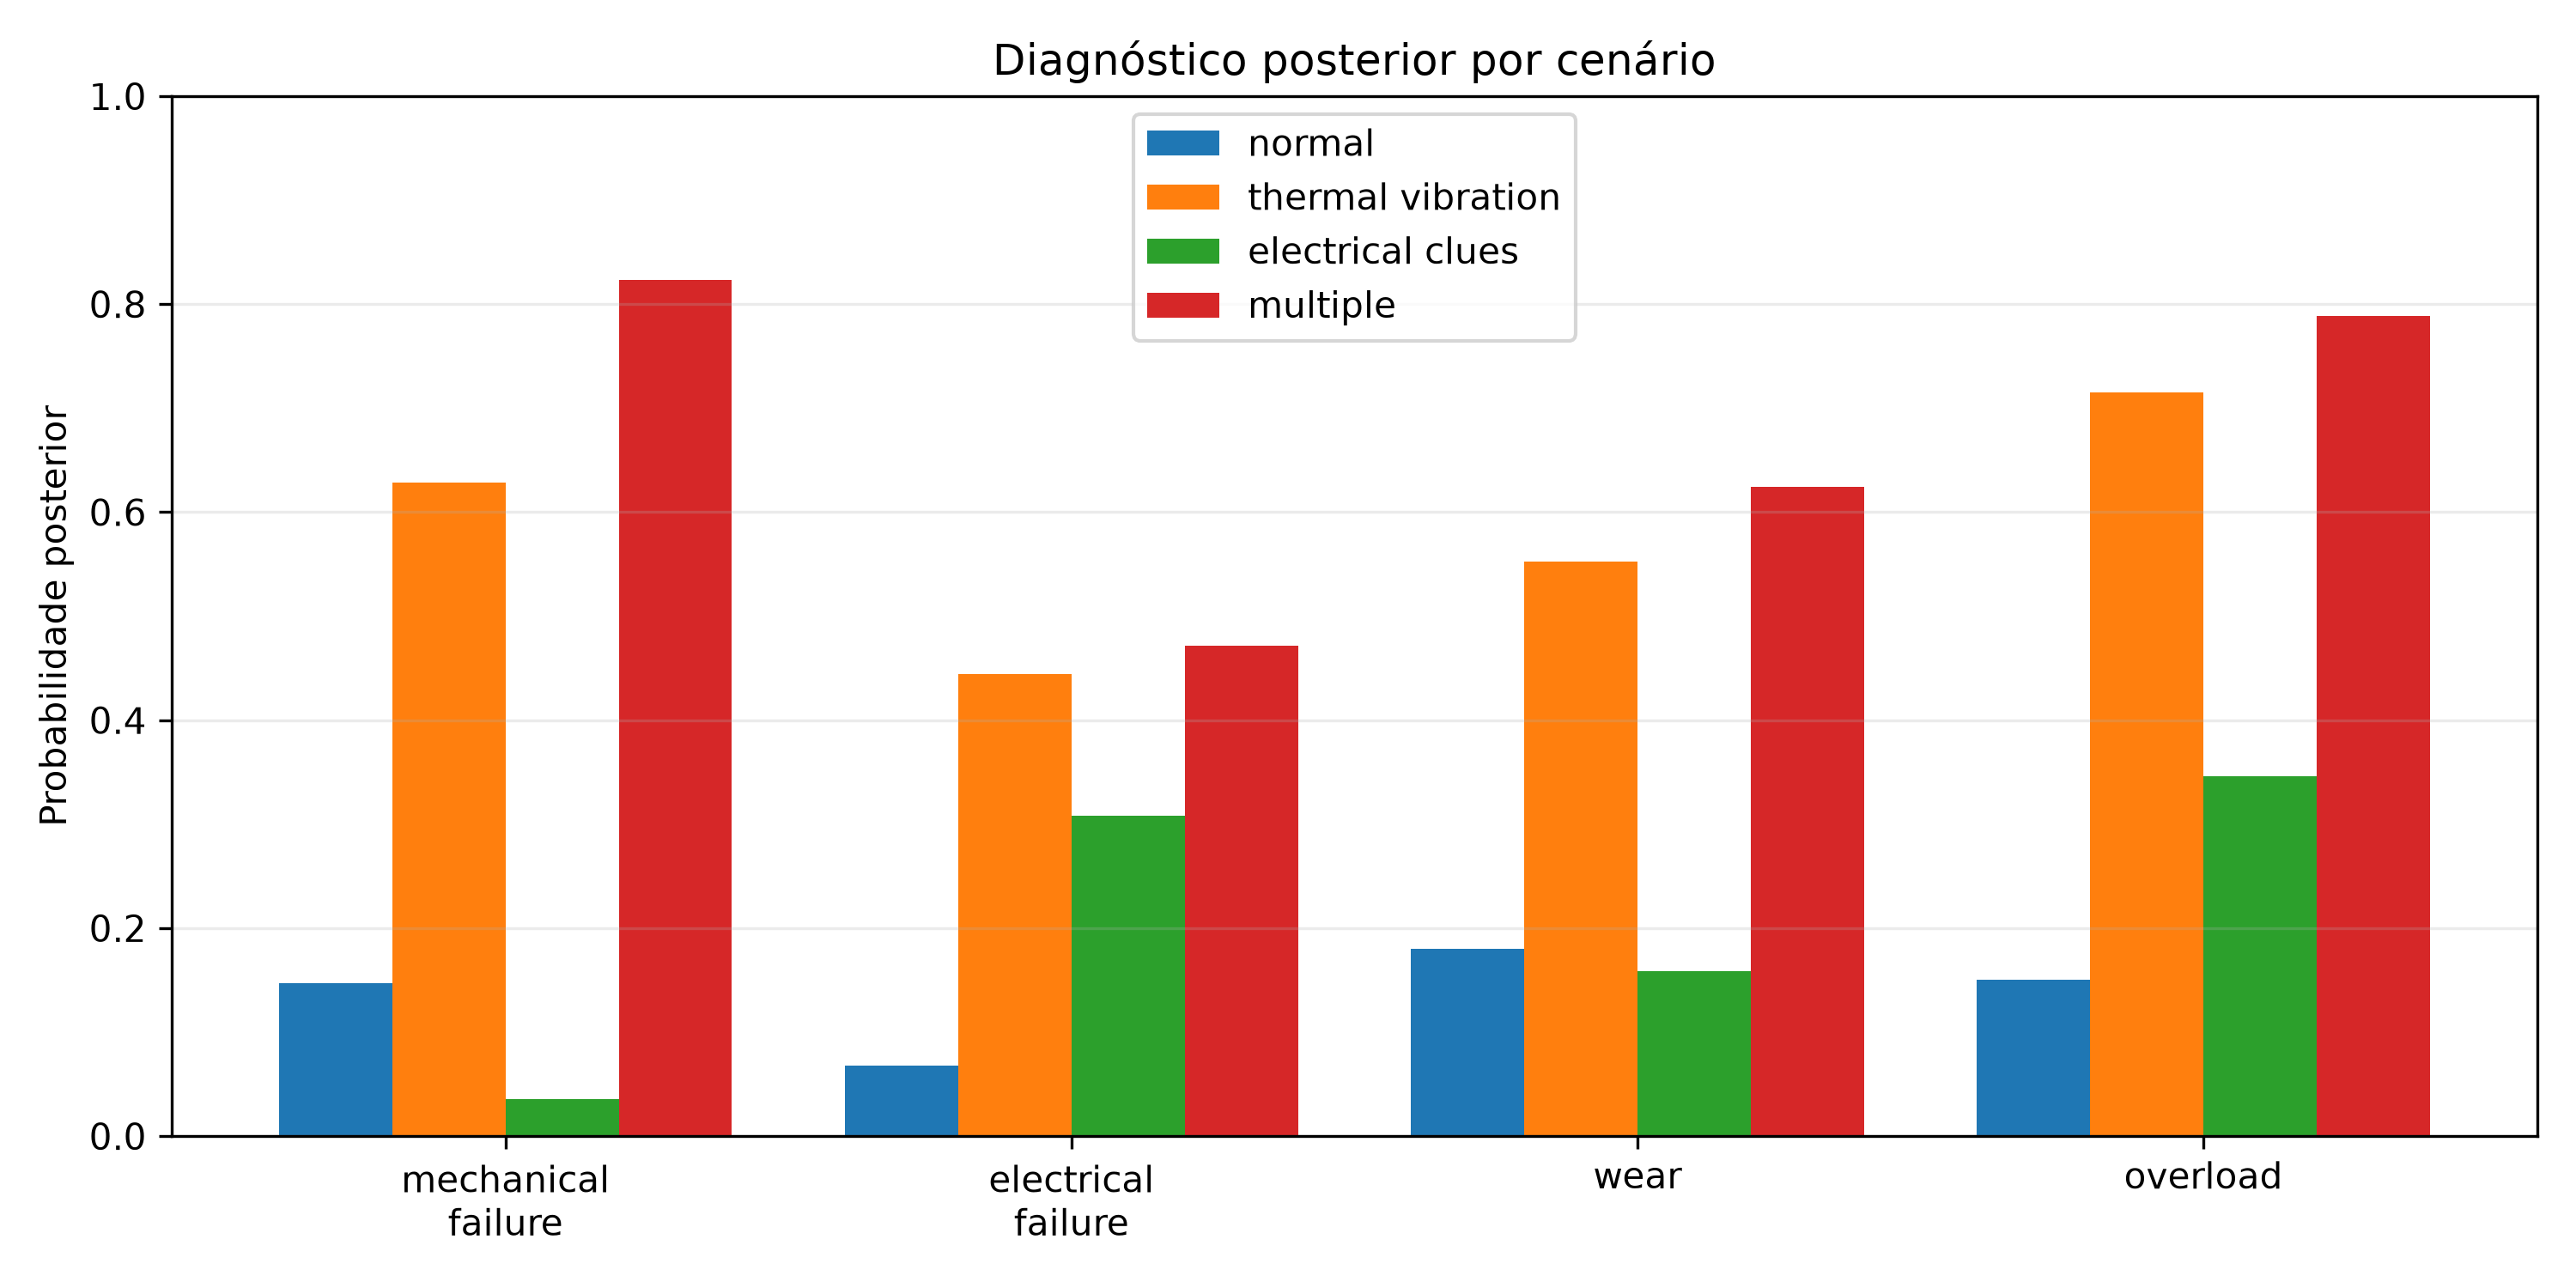
\includegraphics[width=.86\linewidth]{projeto_1_redes_bayesianas/results/posterior_probabilities.png}
\caption{Comparação das probabilidades posteriores nos cenários avaliados.}
\end{figure}

No cenário normal, a falha mecânica apresenta probabilidade posterior de 0,147. Com temperatura e vibração altas, ela sobe para 0,628. Com múltiplas evidências, chega a 0,824. A análise de sensibilidade mostrou que, mantendo temperatura alta, acrescentar vibração alta elevou a probabilidade de falha mecânica em 0,5235. Já o cenário com indícios elétricos, temperatura alta e pressão/vibração normais, favoreceu a hipótese elétrica (0,308) e reduziu a mecânica (0,036), demonstrando que evidências negativas também são informativas.

\section{Projeto 2 — Modelo Markoviano Oculto}
\subsection{Modelagem temporal}
O HMM considera cinco estados ocultos: normal, sobrecarga, desgaste, pré-falha e falha crítica. As observações são seis símbolos discretos que representam combinações de vibração, temperatura e consumo energético. A matriz de transição é persistente e favorece estados próximos, representando degradação gradual. A emissão de cada estado possui um perfil próprio, mas com sobreposição para representar sensores imperfeitos.

Se $A_{ij}=P(S_t=j\mid S_{t-1}=i)$, $B_{jk}=P(O_t=k\mid S_t=j)$ e $\pi_i=P(S_1=i)$, o algoritmo Forward usa
\[
\alpha_t(j)=B_{j,o_t}\sum_i\alpha_{t-1}(i)A_{ij}.
\]
Para evitar underflow, cada vetor $\alpha_t$ é escalonado pela própria soma; a log-verossimilhança é obtida somando os logaritmos dos fatores de escala. O Viterbi foi implementado em logaritmos e conserva probabilidades zero como transições impossíveis. O Baum--Welch usa as responsabilidades $\gamma$ e $\xi$ para atualizar $A$, $B$ e $\pi$ por máxima verossimilhança iterativa.

\subsection{Resultados}
Uma sequência de 180 instantes foi gerada com semente 19 a partir do modelo conhecido. A sequência estimada pelo Viterbi obteve acurácia de \textbf{0,856} e F1 macro de \textbf{0,740}. A maior parte das confusões ocorreu entre estados vizinhos, principalmente desgaste, sobrecarga e pré-falha, o que é coerente com emissões parcialmente sobrepostas.

\begin{figure}[H]
\centering
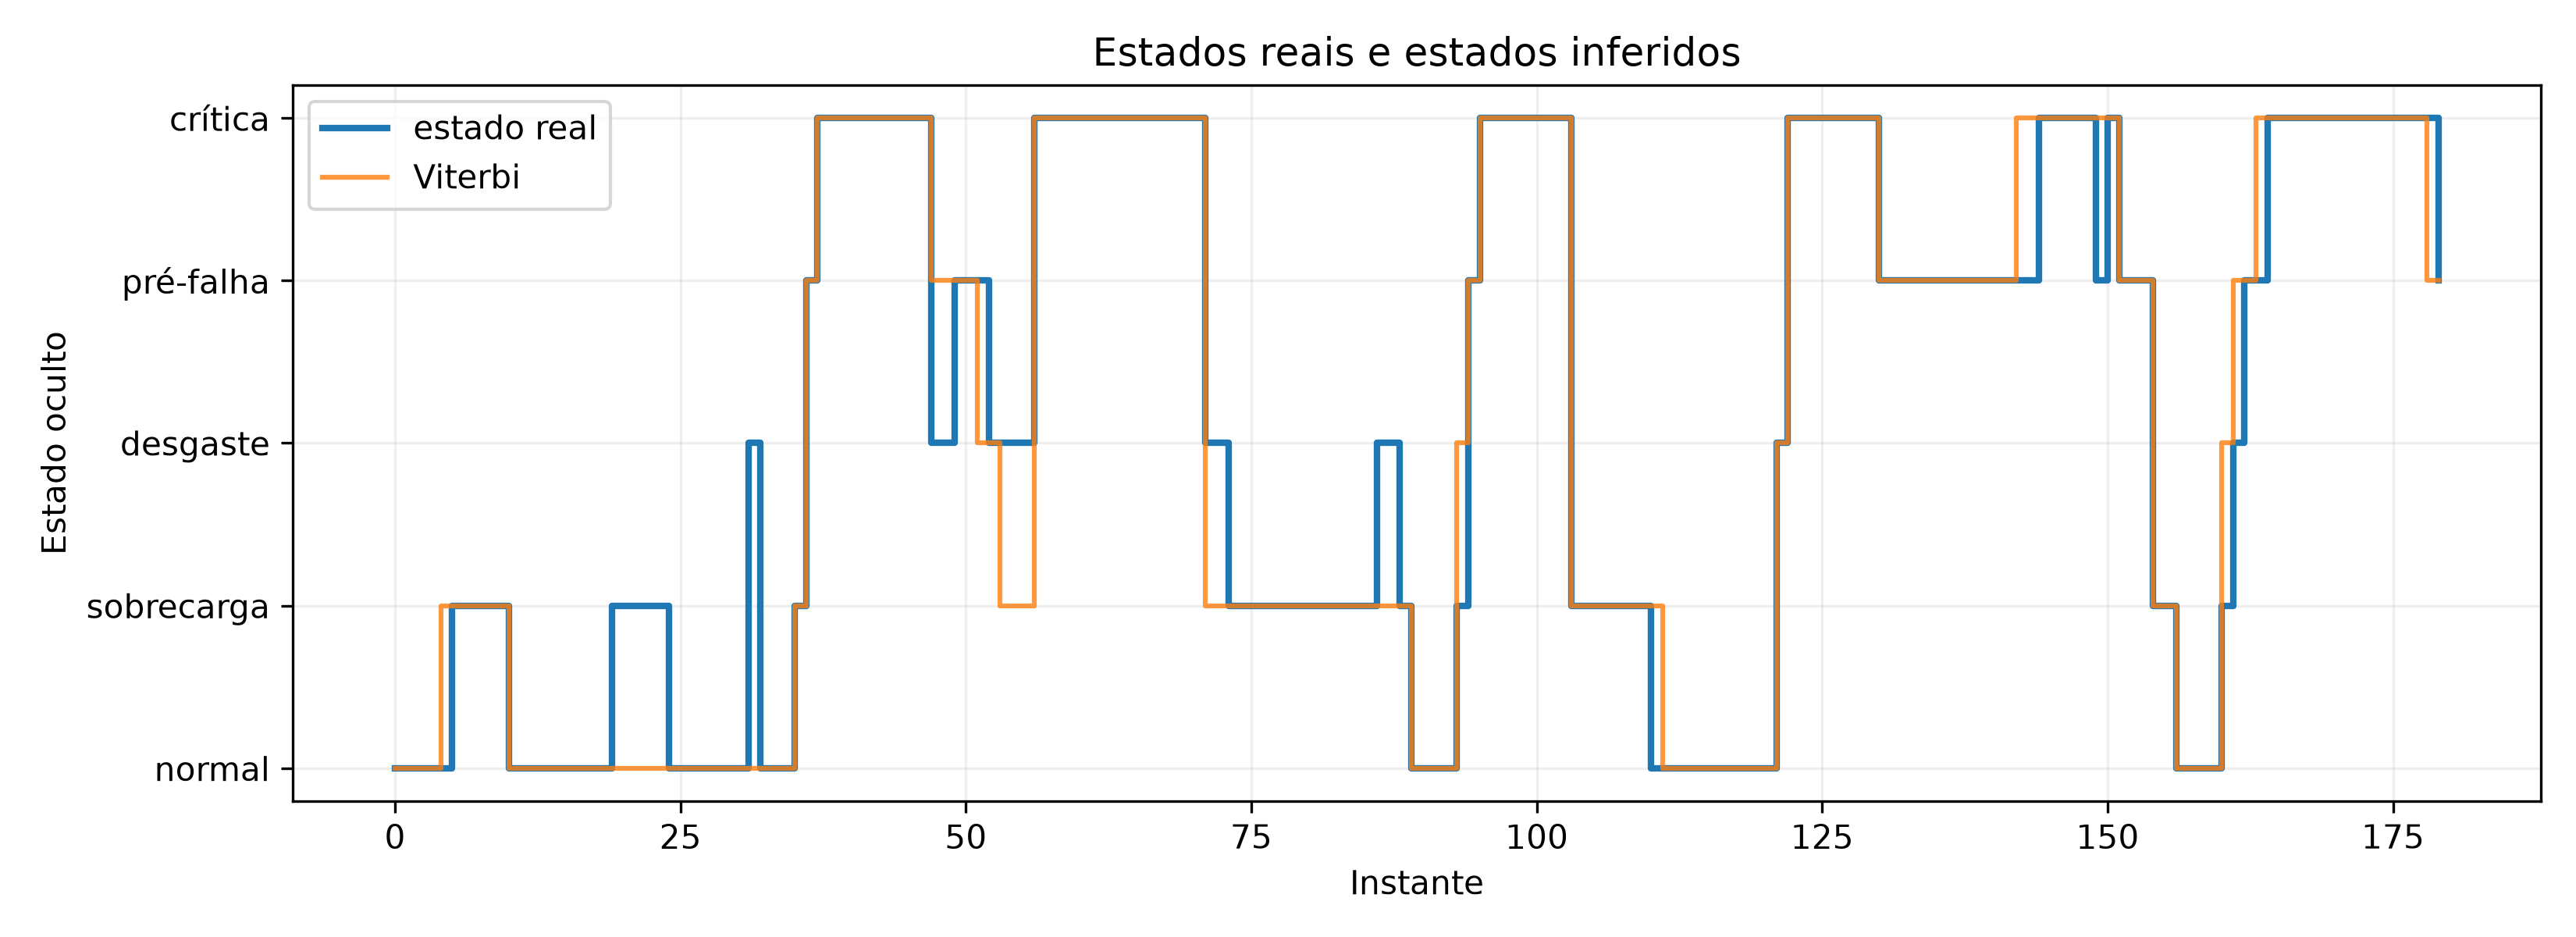
\includegraphics[width=.92\linewidth]{projeto_2_hmm/results/state_comparison.png}
\caption{Estados reais e estados estimados pelo Viterbi.}
\end{figure}

\begin{table}[H]\centering\small
\caption{Matriz de confusão: linhas são estados reais e colunas são estados estimados.}
\begin{tabular}{lrrrrr}
\toprule
 & Normal & Sobrecarga & Desgaste & Pré-falha & Crítica\\
\midrule
Normal & 41 & 2 & 0 & 0 & 0\\
Sobrecarga & 5 & 29 & 2 & 0 & 0\\
Desgaste & 1 & 7 & 2 & 3 & 0\\
Pré-falha & 0 & 0 & 1 & 21 & 4\\
Crítica & 0 & 0 & 0 & 1 & 61\\
\bottomrule
\end{tabular}
\end{table}

Em oito sequências adicionais de 100 símbolos, o Baum--Welch aumentou a log-verossimilhança de $-1179,383$ para $-1160,193$ em 40 iterações. Esse aumento indica melhora do ajuste aos dados, embora não garanta que os estados aprendidos mantenham a mesma interpretação sem uma etapa de identificação dos rótulos.

\begin{figure}[H]
\centering
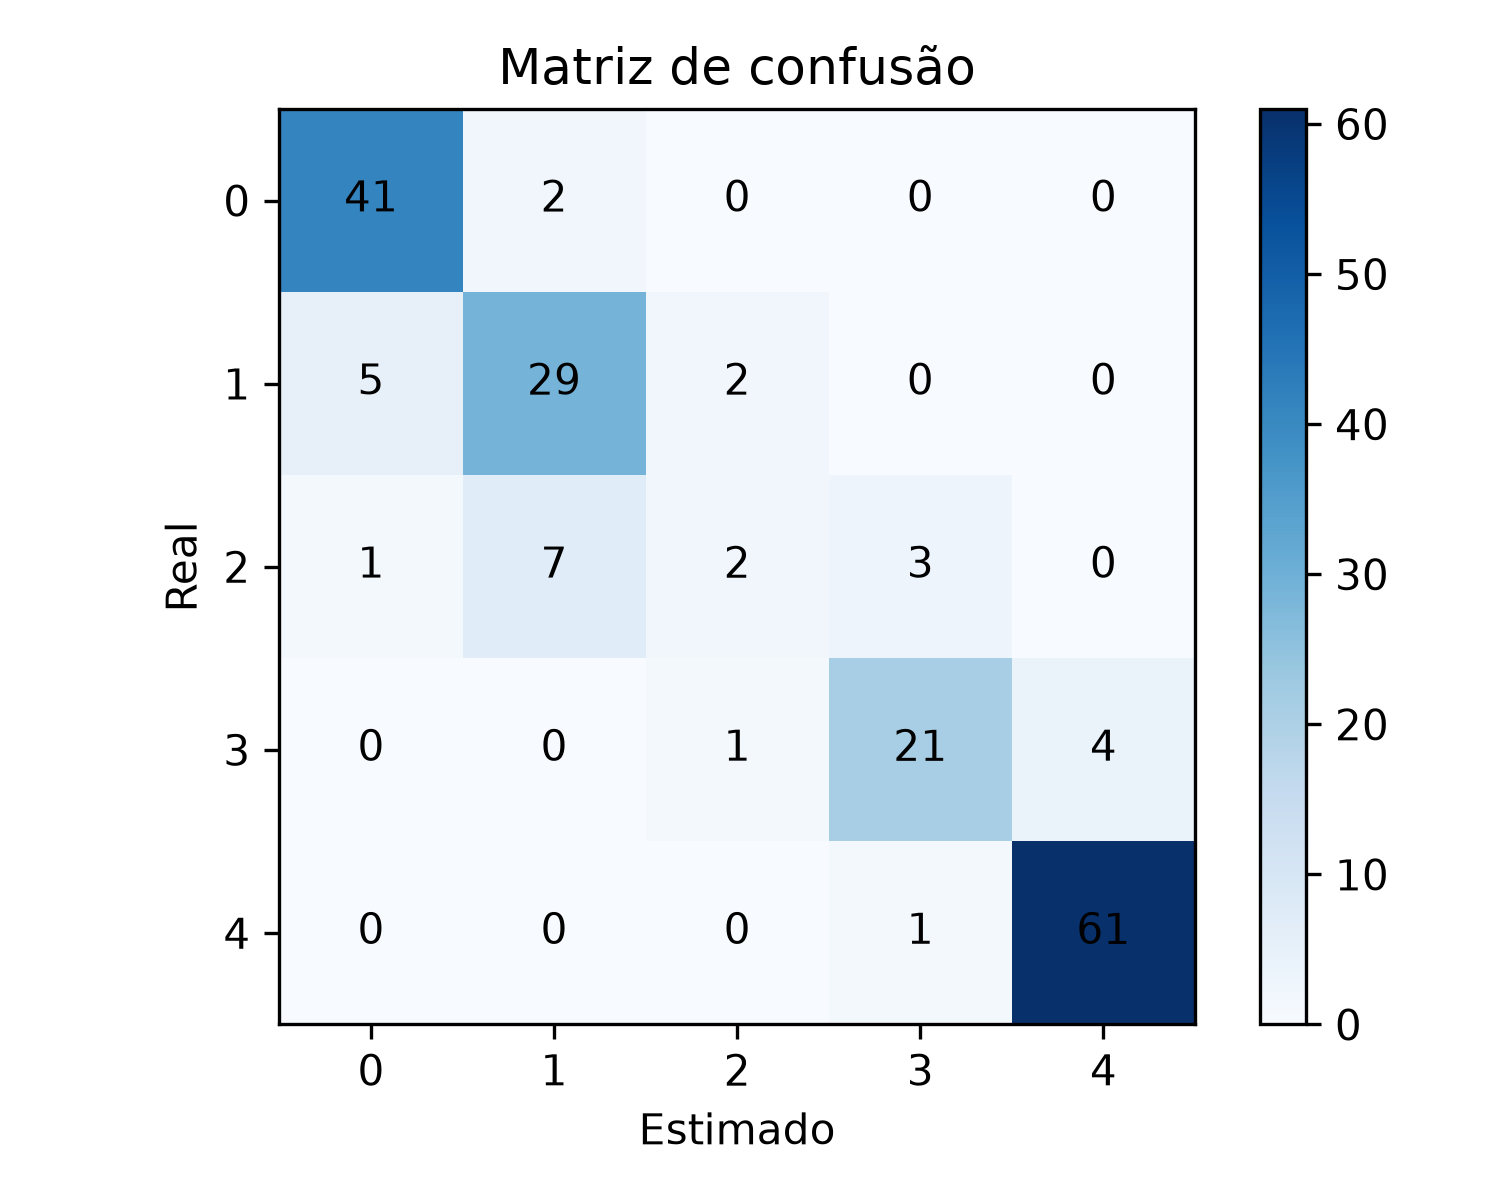
\includegraphics[width=.4\linewidth]{projeto_2_hmm/results/confusion_matrix.png}
\hspace{.06\linewidth}
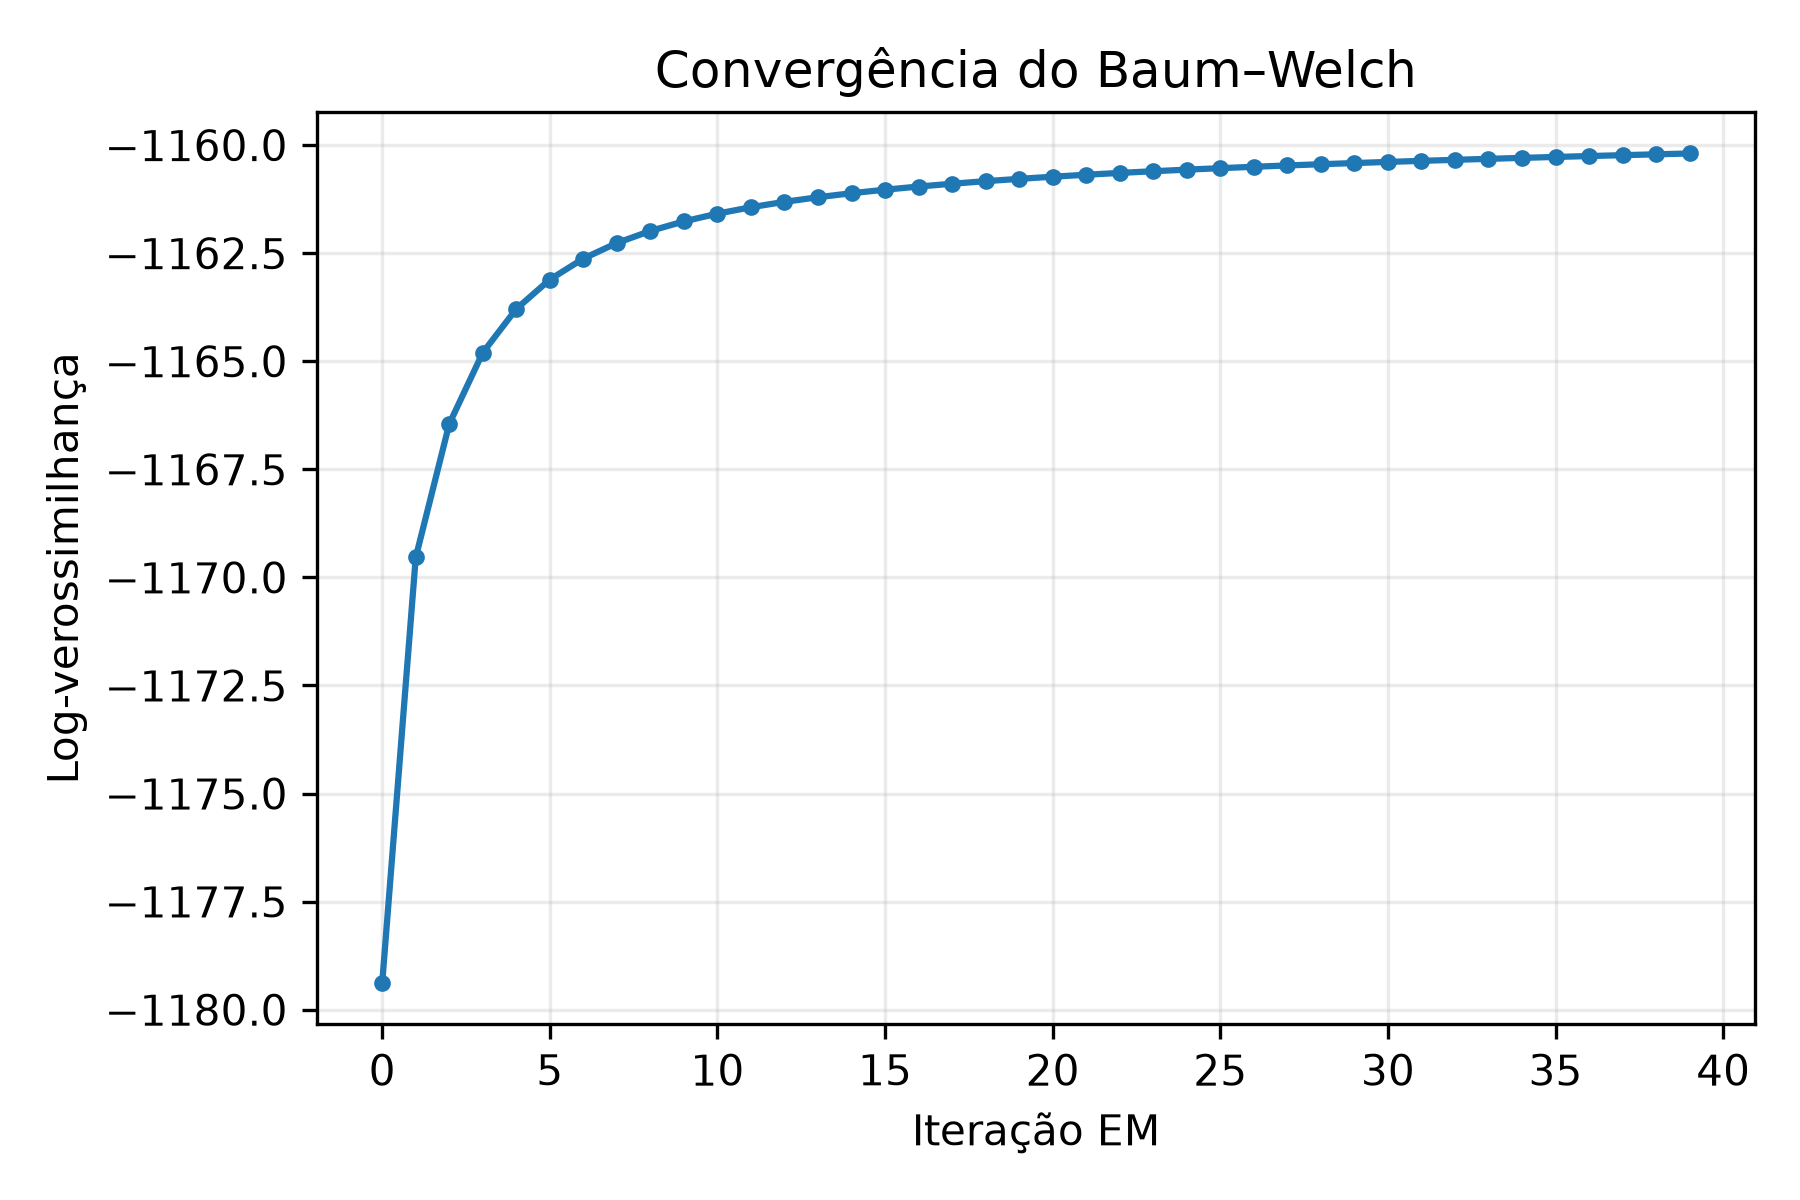
\includegraphics[width=.48\linewidth]{projeto_2_hmm/results/likelihood_analysis.png}
\caption{Matriz de confusão e convergência do Baum--Welch.}
\end{figure}

\section{Projeto 3 — Filtro de Kalman}
\subsection{Modelo dinâmico}
O estado físico é $\mathbf{x}_k=[p_k,v_k]^T$, contendo posição e velocidade. Com $\Delta t=0,5$ s, o modelo quase uniforme é
\[
\mathbf{x}_k=F\mathbf{x}_{k-1}+\mathbf{w}_k,\quad
F=\begin{bmatrix}1&\Delta t\\0&1\end{bmatrix},
\qquad
z_k=H\mathbf{x}_k+v_k,\quad H=[1\ 0].
\]
O processo usa $Q=\operatorname{diag}(0,002;0,01)$ e a medição nominal usa $R=4$. A trajetória foi simulada com posição inicial zero, velocidade inicial 1,2 e perturbação gaussiana de processo.

\subsection{Filtragem}
Na predição:
\[
\hat{x}_{k|k-1}=F\hat{x}_{k-1|k-1},\qquad
P_k^-=FP_{k-1}F^T+Q.
\]
Na atualização:
\[
S_k=HP_k^-H^T+R,\qquad K_k=P_k^-H^TS_k^{-1},
\]
\[
\hat{x}_{k|k}=\hat{x}_{k|k-1}+K_k(z_k-H\hat{x}_{k|k-1}).
\]
Para melhorar a estabilidade numérica, a covariância é atualizada na forma de Joseph:
\[
P_k=(I-K_kH)P_k^-(I-K_kH)^T+K_kRK_k^T.
\]
Na implementação, o ganho é calculado por solução de sistema linear, evitando a inversão explícita de $S_k$.

\subsection{Resultados}
Com semente 23 e 120 amostras, o sensor apresentou RMSE de posição 1,954 e MAE 1,544. Após a filtragem, os valores caíram para RMSE 1,176 e MAE 0,973.

\begin{figure}[H]
\centering
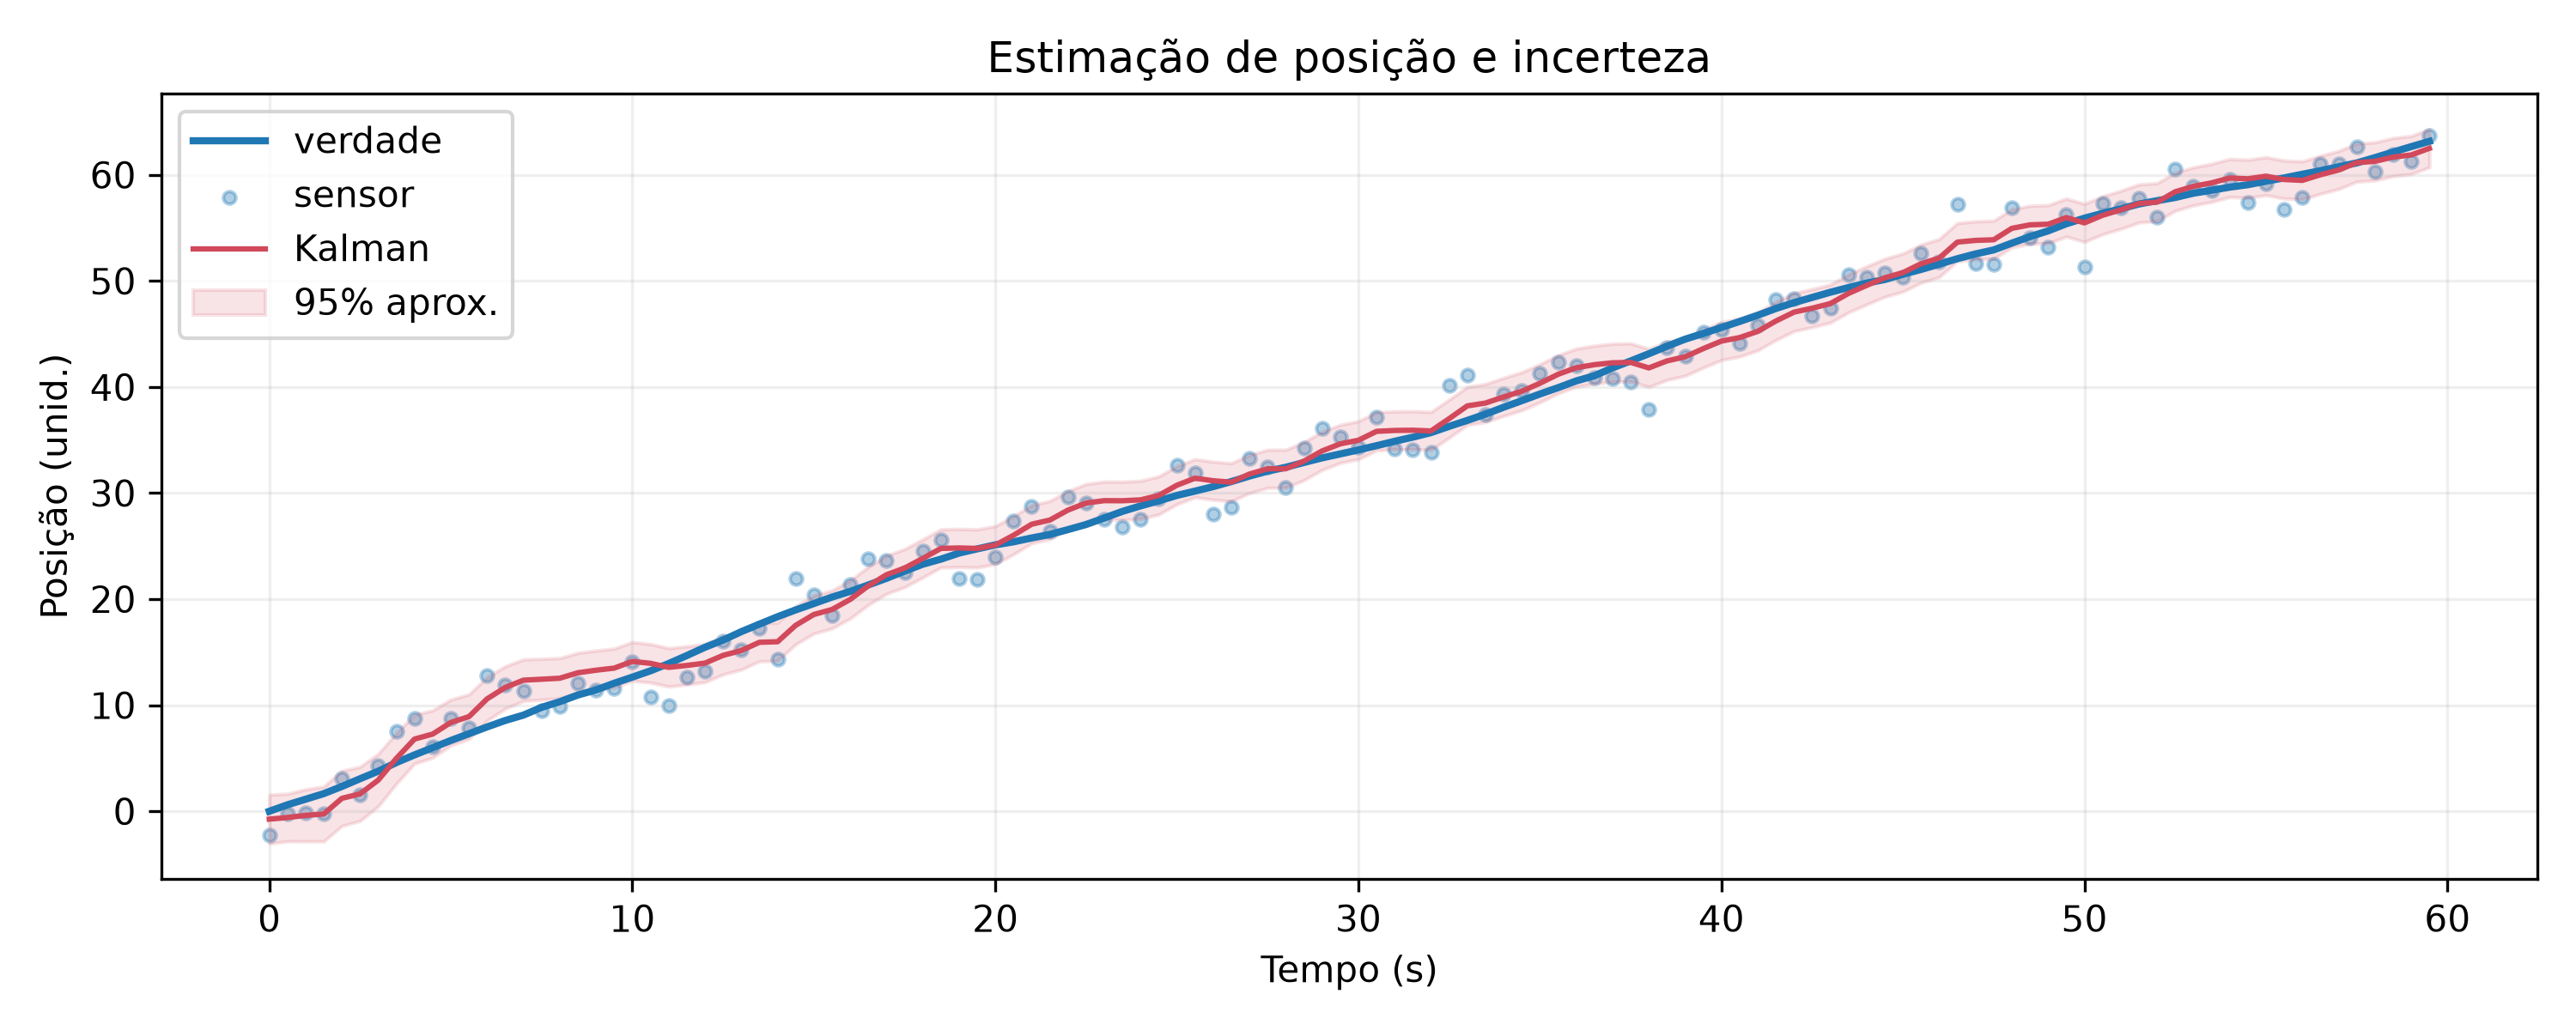
\includegraphics[width=.92\linewidth]{projeto_3_kalman/results/state_estimation.png}
\caption{Trajetória verdadeira, medições, estimativa e incerteza aproximada.}
\end{figure}

\begin{table}[H]\centering\small
\caption{Influência da variância real do ruído de medição.}
\begin{tabular}{rrrrr}
\toprule
Variância $R$ & 0,25 & 1 & 4 & 16\\
\midrule
RMSE do sensor & 0,489 & 0,977 & 1,954 & 3,909\\
RMSE do Kalman & 0,379 & 0,689 & 1,176 & 1,902\\
\bottomrule
\end{tabular}
\end{table}

\begin{figure}[H]
\centering
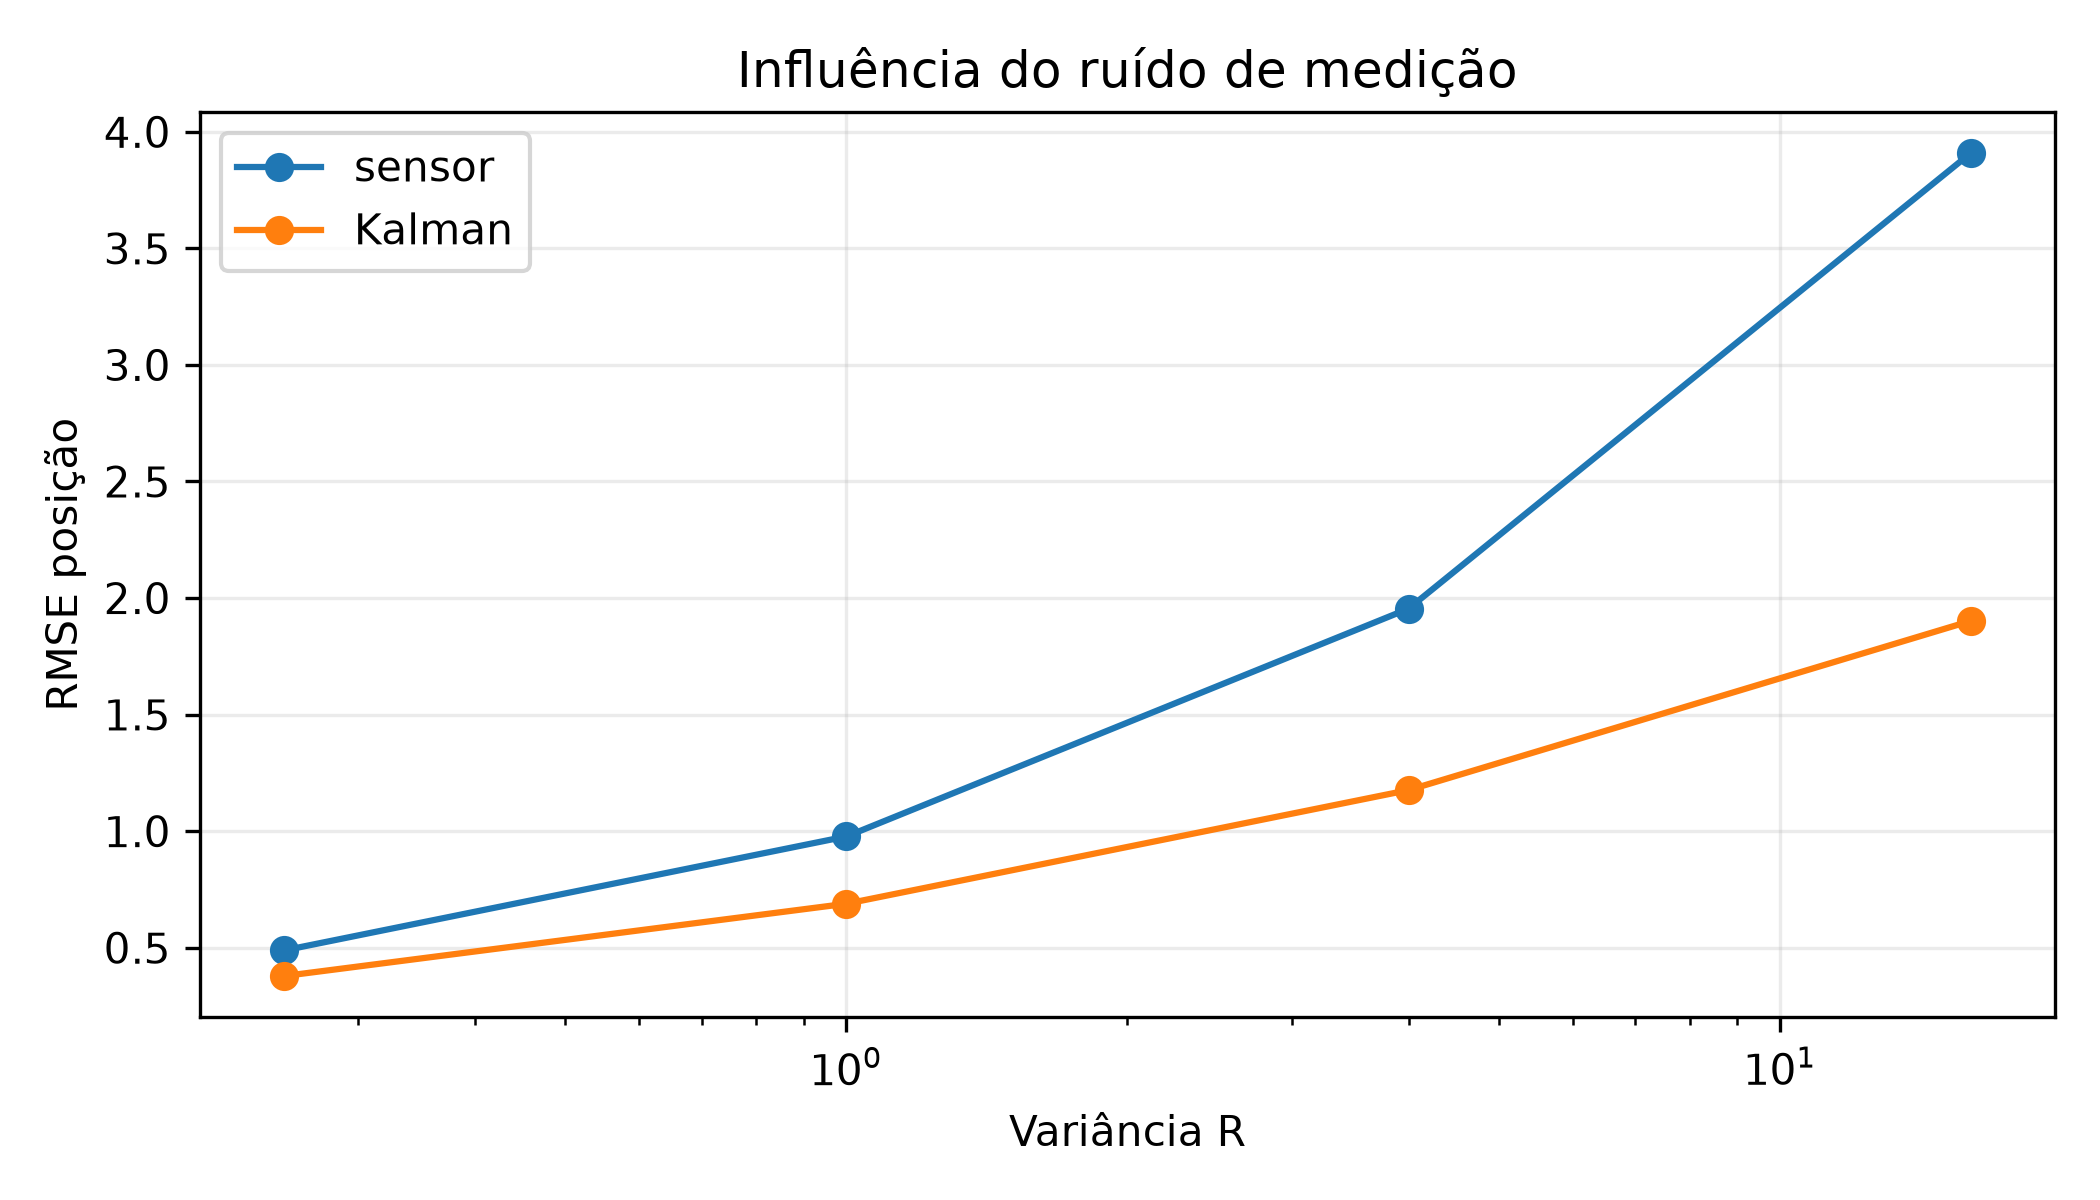
\includegraphics[width=.72\linewidth]{projeto_3_kalman/results/noise_comparison.png}
\caption{Comparação do erro em diferentes níveis de ruído.}
\end{figure}

O filtro manteve vantagem em todos os níveis testados. Quando o ruído verdadeiro tinha variância 4, mas o filtro assumiu incorretamente $R=0,25$, o RMSE foi 1,386, maior que o valor nominal 1,176. Isso mostra que a qualidade depende não apenas do algoritmo, mas também da calibração das covariâncias.

\section{Discussão comparativa}
Os três métodos não são concorrentes diretos; eles modelam incertezas diferentes. A Rede Bayesiana é apropriada para diagnóstico causal e integração de evidências em um instante. O HMM representa dependência temporal discreta e permite reconstruir uma trajetória de estados ocultos. O Kalman é adequado para variáveis contínuas em sistemas dinâmicos aproximadamente lineares, produzindo também uma covariância de incerteza.

\begin{table}[H]\centering
\caption{Síntese das contribuições e limitações.}
\begin{tabularx}{\linewidth}{lXX}
\toprule
Método & Principal contribuição & Limitação observada\\
\midrule
Rede Bayesiana & Inferência explicável de causas e falhas a partir de evidências & Enumeração cresce exponencialmente; CPTs dependem de conhecimento/calibração\\
HMM & Identificação de estados ocultos e evolução temporal & Depende do conjunto de estados e da separação das emissões\\
Kalman & Estimação contínua suavizada com incerteza explícita & Pressupõe dinâmica linear e ruídos adequadamente modelados\\
\bottomrule
\end{tabularx}
\end{table}

Uma arquitetura industrial realista poderia combinar os três resultados: o Kalman filtraria sinais contínuos, o HMM transformaria sequências em estados operacionais e a Rede Bayesiana integraria o estado atual com evidências causais para priorizar falhas e ações de manutenção. Essa composição deve ser feita com cuidado para evitar contar duas vezes a mesma evidência.

\section{Validação, reprodutibilidade e limitações}
Os códigos foram executados após as alterações finais e os testes automatizados passaram com 7 casos. Foram verificadas: sintaxe dos módulos, normalização das matrizes do HMM após Baum--Welch, simetria e semidefinição positiva das covariâncias do Kalman, completude das CPTs e geração dos arquivos de métricas e figuras. Os três relatórios auxiliares individuais permanecem no repositório, mas este documento é o relatório geral principal.

As conclusões são limitadas pelo uso de dados sintéticos e por parâmetros especificados manualmente. Os resultados não substituem validação em dados históricos de sensores, registros de manutenção e diferentes regimes de operação. Em continuidade, seria importante estimar CPTs e emissões a partir de dados reais, testar HMMs com estados não estacionários, usar filtros robustos contra outliers e comparar a enumeração com eliminação de variáveis em redes maiores.

\section{Conclusão}
O portfólio demonstrou três perspectivas complementares para tratar incerteza em sistemas industriais. A Rede Bayesiana quantificou diagnósticos e respondeu de forma sensível a evidências combinadas. O HMM recuperou estados ocultos com acurácia de 0,856 e mostrou aumento da verossimilhança durante o aprendizado. O Filtro de Kalman reduziu substancialmente os erros de posição e evidenciou o impacto de uma hipótese incorreta sobre o ruído.

Mais importante que os valores isolados, os experimentos evidenciam as hipóteses de cada algoritmo. A escolha do método deve acompanhar a natureza da incerteza: dependências causais, evolução temporal discreta ou dinâmica contínua. O código, os resultados e as figuras foram organizados para permitir reprodução e inspeção dos cálculos.

\section*{Referências}
\begin{enumerate}
\item BAUM, L. E. et al. A maximization technique occurring in the statistical analysis of probabilistic functions of Markov chains. \textit{The Annals of Mathematical Statistics}, v. 41, n. 1, p. 164--171, 1970. DOI: 10.1214/aoms/1177697196.
\item KALMAN, R. E. A new approach to linear filtering and prediction problems. \textit{Journal of Basic Engineering}, v. 82, n. 1, p. 35--45, 1960. DOI: 10.1115/1.3662552.
\item KOLLER, D.; FRIEDMAN, N. \textit{Probabilistic Graphical Models: Principles and Techniques}. MIT Press, 2009.
\item RABINER, L. R. A tutorial on hidden Markov models and selected applications in speech recognition. \textit{Proceedings of the IEEE}, v. 77, n. 2, p. 257--286, 1989. DOI: 10.1109/5.18626.
\item RUSSELL, S.; NORVIG, P. \textit{Artificial Intelligence: A Modern Approach}. 4. ed. Pearson, 2021.
\item SIMON, D. \textit{Optimal State Estimation: Kalman, H Infinity, and Nonlinear Approaches}. Wiley, 2006.
\end{enumerate}
\end{document}
